\section{DBCheck}
The author’s model checking project was named NuSMV. The models used in this work are all variations of a general concurrency model. This model consists of a process module and memory cell module. At this point, all the models are implemented with 2 processes and 2 memory cells. 


\begin{figure}[H]
	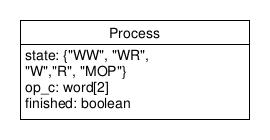
\includegraphics[width=\linewidth]{dbcheck_model.jpg}
\end{figure}

This intent of the process module is to represent the action of a database transaction thread. For the purposes of this work, the memory cell only implements the lock for a given database resource. Depending on the variations of the model’s implementation, the internal logic will differ and some execute with respect to different input or internal parameters.

\subsection{DBCheck Models}
For the testing purposes, DBCheck currently has 4 main model classes. These are a Strict 2PL model, a Conservative 2PL model, a naive model, and a final additional model, C1. Each of the models has 2 versions, a 2 operation schedule version and a 4 operation schedule version. 

\subsection{DBCheck Specs}
DBCheck Specs
In testing the model’s adherence to the serializability property or other properties of an ACID DBMS, different levels of rigor may be used as to the result. Also, the generality of the model allows for different granularities. In a practical implementation,  the specifications may involve the literal semantics of the data. In the testing at this stage of DBCheck, the specifications are situated around three different possible forms of occurrence in a non-serializable model. These are WW errors, WR errors and RW errors. A stated problem with Strict 2PL is that it may have issues with deadlock. For this reason, a deadlock specification is also used. The specifications are shown with their CTL syntax.
\begin{enumerate}
\item $AG ((p1.state[i] = “W”)  \implies (AG \neg( \negP1.finished \land p2.state[i]=”W”))$
This says that in the model that if a process p1 has a write operation on resource i, then in every following state it cannot be true that p1 has not finished and p2 has a write operation on resource i. This would correspond to a blind write. 
\item $AG ((p1.state[i] = “R”)  \implies (AG \neg(\neg P1.finished \land p2.state[i]=”W”))$
This says that in the model that if a process p1 has a read operation on resource i, then in every following state it cannot be true that p1 has not finished and p2 has a write operation on resource i.
\item $AG ((p1.state[i] = “W”)  \implies (AG \neg(\neg P1.finished \land p2.state[i]=”R”))$
This says that in the model that if a process p1 has a write operation on resource i, then in every following state it cannot be true that p1 has not finished and p2 has a read operation on resource i.
\end{enumerate}

These properties are all expected to hold within 2PL. This should be true with respect to both Strict 2PL and Conservative 2PL. However, their implication to serializability rests on order assumptions. DBCheck does not have a serializable order defined for all models. For the naive model and strict 2PL there is no order defined for the model. In C1 and C2PL, the models do have an order defined.  The two final properties are a property for 2PL and the deadlock property. 

\begin{enumerate}
	\item $AF (p1.finished \land p2.finished)$

	This property just asserted that the schedules always finish. Later in the results, an example is shown of a conuterexample to this specification for Strict 2PL which shows a deadlock situation.

	\item $G (( acell.lock = 1 \land X ( acell.lock = 0)) \implies X(G \neg (acell.lock = 1)))$

		This property, which is actually defined separety for the model based on the lock definition, expresses that for each process, if it has released a lock it doesn't reqaquire it.

\end{enumerate}

This is defined loosely as 
AF ( p1.finished \& p2.finished)
The meaning of this is that in all states there exists a future state where both processes have finished.


